\documentclass[12pt,leqno]{amsart}
\usepackage{pgfplots}       % it also load tikz package
\pgfplotsset{compat=1.17}   
\usetikzlibrary{arrows.meta}
\usepackage{tikz}
\usepackage{tcolorbox}
\usetikzlibrary{shapes.geometric, arrows}
\tikzstyle{startstop} = [rectangle, rounded corners, minimum width=3cm, minimum height=1cm,text centered, draw=black, fill=red!30]
\tikzstyle{io} = [trapezium, trapezium left angle=70, trapezium right angle=110, minimum width=4cm, minimum height=1cm, text centered, draw=black, fill=blue!30]
\tikzstyle{process} = [rectangle, minimum width=3cm, minimum height=1cm, text centered, draw=black, fill=orange!30]
\tikzstyle{decision} = [diamond, minimum width=3cm, minimum height=1cm, text centered, draw=black, fill=green!30]
\tikzstyle{arrow} = [thick,->,>=stealth]
\usepackage{tcolorbox}
\usepackage{caption}
\usepackage[colorlinks=true,
            citecolor={black}]{hyperref}
\usepackage{lipsum} % added for generating a dummy text, 
                    % not needed in real document
\usepackage{fancyvrb}

\begin{document}
%\lipsum[1]  % dummy text
%\begin{tcolorbox}[colback=white]
\section{\textbf{Extraction of public administration data from official document}}
The following modules were used to perform a Named Entity Recognition of data from Public Administration documents(mostly tenders).
Those data describe the certifications that a company is required to have to apply for a tender; such certification in Italy are called SOA-certifications(S.O.A.: in Italian "Società degli Organismi di Attestazione", in English "Certification Organizations' Society ").
The modules of this repository were built and used to extract  certifications data from documents.
\newline
\paragraph{\textbf{Modules}}
\begin{enumerate}
\item{\textbf{NER regex:}}
python script that extracts SOA data with the usage of regular expressions;
\item{\textbf{dataset splitter:}} takes a gold.json1 file describing the ground truth; divides it into many labelled sentences, distributing them to the train/dev/test bins;
It's a necessary step for the setup of a NER task in spacy;
\item{\textbf{NER SpaCy:}} bash scripts to initialize, train, debug and evaluate the neural network with the usage of the Spacy library;
\item{\textbf{scorer for regex-extracted data:}} takes in input some regex-extracted soa data (v1, v2 or v3, retrieved by using different regex) and scores them by comparing them to the ground truth;
\item{\textbf{json to csv:}} helper script to convert Spacy-scores from json format to csv format;
\end{enumerate}
documented\_outputs: results of the modules with the real data.
\newpage
\paragraph{\textbf{1.NER regex:}}
\begin{itemize}
\item{\textbf{what's inside:}}
it contains the main script *ner\_regex.py* and the *Dataset* folder.
The Dataset folder is provided with an example *"soa.csv" input file* containing documents.
\item{\textbf{usage:}}
The user can just execute the script ner\_regex.py.
This module is meant to find text-instances of SOA data and to label them.
\item{\textbf{output:}}
a .json1 file containing annotations that describe the retrieved entities.
\end{itemize}
%REGEX NER
	\begin{figure}[ht] % placed here or on the top of page
		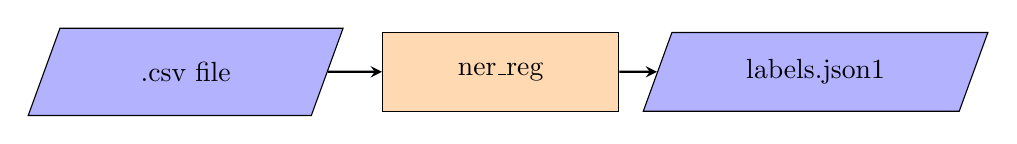
\begin{tikzpicture}[node distance=4cm]
			\node (start) [io] {.csv file};
			\node (module) [process, right of=start] {ner\_reg};
			\node (stop) [io, right of=module] {labels.json1};
			\draw (0,0) [arrow] (start) -- (module);
			\draw [arrow] (module) -- (stop);
		\end{tikzpicture}
		\caption{Module 1} % caption
		%\label{fig:diagram}             % for referencing of figure, key select as you wish
	\end{figure}
%\lipsum[2]  % dummy textù


\paragraph{\textbf{S2.Dataset splitter}}
\begin{itemize}
\item{\textbf{input:}}
The gold.json1 file is an example of **Ground Truth**. This module takes the gold.json1 and
divides creates the docbins that will be used later on for building a NN.
\item{\textbf{usage:}}
Execute the dataset\_splitter.py script
\item{\textbf{output:}}
Train.spacy, Dev.spacy, Test.spacy.
\end{itemize}
\begin{figure}[ht] % placed here or on the top of page
    % DATASET SPLITTER
    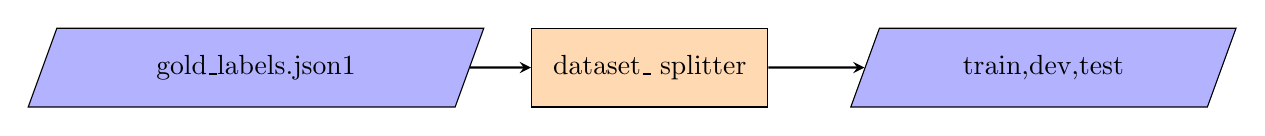
\begin{tikzpicture}[node distance=5cm]
        \node (start) [io] {gold\_labels.json1};
        \node (module) [process, right of=start] {dataset\_ splitter};
        \node (stop) [io, right of=module] {train,dev,test};
        \draw [arrow] (start) -- (module);
        \draw [arrow] (module) -- (stop);
    \end{tikzpicture}
    \caption{Module 2} % caption
    %\label{fig:diagram}             % for referencing of figure, key select as you wish
    \end{figure}
%\lipsum[2]  % dummy text

\newpage
\paragraph{\textbf{S3.NER spaCy}}
\begin{itemize}
\item{\textbf{inputs: }}the module needs the docbins **train.spacy**,**dev.spacy**,**test.spacy** produced by the Dataset Splitter Module.
\item{\textbf{usage: }}
1. execute script 3.0-retrieve-inputs.sh, it will copy the spacy file from the previous module 
2. 3.1-train.sh: trains a neural network
3. 3.2-debug.sh: retrieves info on how experienced the NN is.
4. 3.3-evaluate.sh: tests the NN with the test data of the test.spacy file
\item{\textbf{outputs: }}
NN model with debug information and testing results.
\end{itemize}
% SPACY NER 
\begin{figure}[ht] % placed here or on the top of page
    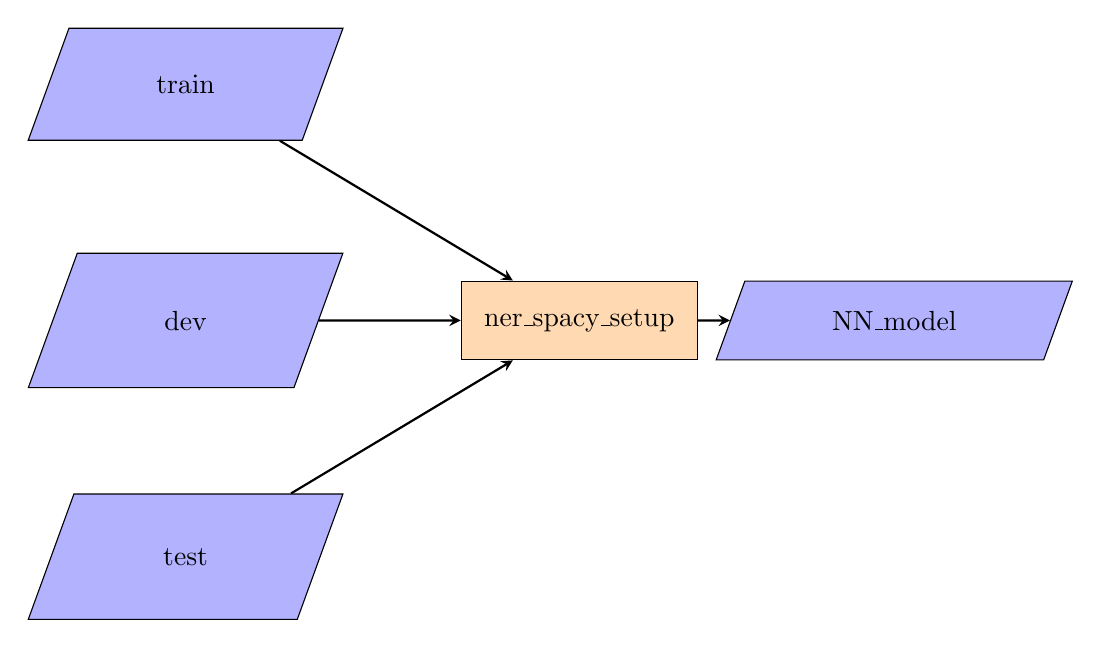
\begin{tikzpicture}[node distance=1cm]
        \node (train) [io] {train};
        \node (dev) [io, below of=train, node distance=3cm] {dev};
        \node (test) [io, below of=dev, node distance=3cm] {test};
        \node (module) [process, right of=dev, node distance=5cm] {ner\_spacy\_setup};
        \node (stop) [io, right of=module, node distance=4cm] {NN\_model};
        \draw [arrow] (train) -- (module);
        \draw [arrow] (dev) -- (module);
        \draw [arrow] (test) -- (module);
        \draw [arrow] (module) -- (stop);
    \end{tikzpicture}
    \caption{Module 3} % caption
    %\label{fig:diagram}             % for referencing of figure, key select as you wish
    \end{figure}
%\lipsum[2]  % dummy text



\paragraph{\textbf{wip model usage}}
\lipsum[2]  % dummy text
\begin{figure}[ht]
% MODEL USAGE
    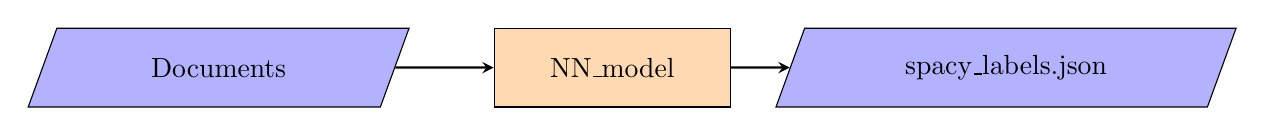
\begin{tikzpicture}[node distance=5cm]
        \node (start) [io] {Documents};
        \node (module) [process, right of=start] {NN\_model};
        \node (stop) [io, right of=module] {spacy\_labels.json};
        \draw [arrow] (start) -- (module);
        \draw [arrow] (module) -- (stop);
    \end{tikzpicture}
\end{figure}


\newpage
\paragraph{\textbf{Scorer}}
\begin{itemize}
\item{\textbf{inputs: }}
gold.json, describes the Ground Truth
\item{\textbf{usage: }}
1. 4.0-retrieve-inputs.sh: retrieves the ner.json1 produced by the  NER


2. scorer\_for\_regex\_extracted\_data***: scores the  ner.json1 by comparing it to the gold.json
\item{\textbf{outputs: }}output-cat-class.json: scores for every category item and classification item
\end{itemize}
\begin{figure}[ht]
% SCORER
    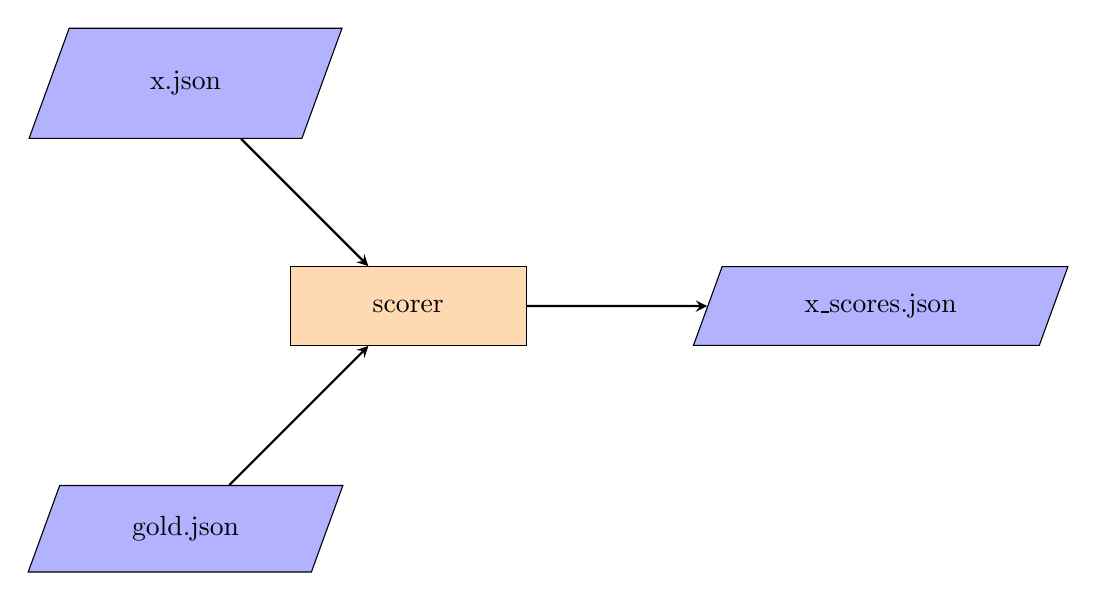
\begin{tikzpicture}[node distance=4cm]
        \node (x) [io] {x.json};
        \node (module) [process, below right of=x] {scorer};
        \node (gold) [io, below left of=module] {gold.json};
        \node (scores) [io, right of=module, node distance=6cm] {x\_scores.json};
        \draw [arrow] (x) -- (module);
        \draw [arrow] (gold) -- (module);
        \draw [arrow] (module) -- (scores);
    \end{tikzpicture}
\end{figure}
%\lipsum[2]  % dummy text


\paragraph{\textbf{Json to csv}}
\begin{itemize}
\item{\textbf{usage: }}put here the score file derived from the scorer output
\item{\textbf{run: }}json\_to\_csv.py 
\item{\textbf{output: }}csv\_tables/ner\_results.csv, describes the scores in a tabular form
\end{itemize}
\begin{figure}[ht]
% JSON TO CSV
    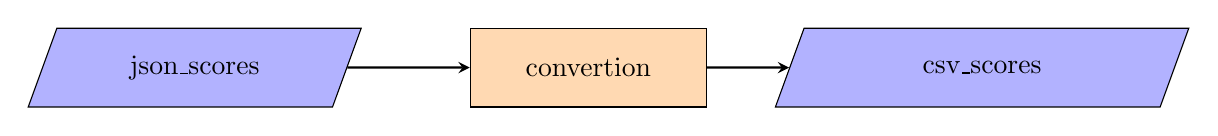
\begin{tikzpicture}[node distance=5cm]
        \node (start) [io] {json\_scores}; %{Input};
        \node (module) [process, right of=start] {convertion};
        \node (stop) [io, right of=module] {csv\_scores}; %{Output};
        \draw [arrow] (start) -- (module);
        \draw [arrow] (module) -- (stop);
    \end{tikzpicture}
\end{figure}
%\lipsum[2]  % dummy text

%\end{tcolorbox}
%For further explanation see figure \ref{fig:diagram} \dots % referencing of figure
\end{document}